% Nallino, Part I p. 256: the figure after Almagest II, 12, redrawn from the print: the meridian ABGD, the horizon
% BED, the vertical circle from the zenith A through the Moon H and E to G, the ecliptic from Z through H and T
% (the ascendant) to the meridian, and the bold italic letters. Measured on the scan (_intake/latin/tools/fig256).
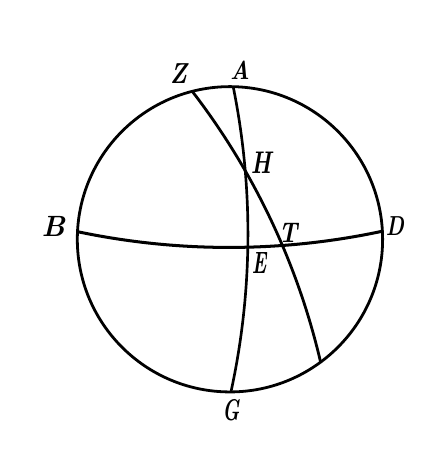
\begin{tikzpicture}[x=0.9964pt,y=-0.9964pt,line cap=butt,every node/.style={font=\fontsize{11}{11}\bfseries\itshape\selectfont,inner sep=0pt}]
\useasboundingbox (0,0) rectangle (139.00,143.50);
\draw[line width=1.01pt] (73.36,76.74) circle[radius=55.36];  % the meridian ABGD
\draw[line width=1.09pt] (18.07,73.98) arc[start angle=101.89,end angle=77.94,radius=266.44];
\draw[line width=0.96pt] (74.53,21.39) arc[start angle=-11.44,end angle=12.28,radius=269.33];
\draw[line width=1.01pt] (59.69,23.09) arc[start angle=-37.57,end angle=-13.14,radius=256.76];
\node at (54.71,16.64) {\normalfont\fontsize{11}{11}\bfseries\itshape\selectfont \resizebox{6.18pt}{7.17pt}{Z}};
\node at (76.99,15.68) {\normalfont\fontsize{11}{11}\bfseries\itshape\selectfont \resizebox{7.09pt}{6.44pt}{A}};
\node at (84.65,49.12) {\normalfont\fontsize{11}{11}\bfseries\itshape\selectfont \resizebox{7.31pt}{7.76pt}{H}};
\node at (9.30,72.14) {\normalfont\fontsize{11}{11}\bfseries\itshape\selectfont \resizebox{8.47pt}{7.27pt}{B}};
\node at (133.16,71.80) {\normalfont\fontsize{11}{11}\bfseries\itshape\selectfont \resizebox{6.54pt}{6.82pt}{D}};
\node at (94.38,74.42) {\normalfont\fontsize{11}{11}\bfseries\itshape\selectfont \resizebox{6.78pt}{7.04pt}{T}};
\node at (83.97,85.16) {\normalfont\fontsize{11}{11}\bfseries\itshape\selectfont \resizebox{5.25pt}{7.65pt}{E}};
\node at (73.69,138.72) {\normalfont\fontsize{11}{11}\bfseries\itshape\selectfont \resizebox{6.22pt}{7.42pt}{G}};
\end{tikzpicture}
